\chapter{DATA ANALYSIS AND RESULTS}
\label{sec:data_analysis_results}

\section{Data Analysis Plan}

\subsubsection*{Motivation and scope}

The primary output of the MIRAGE post-flight analysis is a quality-controlled vertical methane concentration profile with associated uncertainty bounds, expressed as a function of the altitude. Defining this output early in the design process ensures that the on-board data acquisition, storage format, and sensor operating modes are tailored to produce data that can be systematically processed into a scientifically useful result.\\
Balloon-borne in-situ greenhouse gas profiling missions such as AMULSE \cite{Khair2017} have demonstrated that a well defined post flight data analysis pipeline, encompassing ingestion calibration correction, quality flagging and comparison against independent reference sources, is essential for extracting reliable concentration profiles from raw sensor data. The AMULSE experiment, which used \gls{tdlas}, employed a comparable processing chain to validate satellite retrieval products from IASI. While MIRAGE operates using a fundamentally different measurement method (\gls{ndir} instead of TDLAS), its overall pipeline architecture follows a similar logic: raw detector output must be corrected for environmental conditions, filtered for measurement artifacts, and validated against independent data before scientific conclusions can be drawn.\\
The pipeline directly supports the experiment objectives defined in Table \tref{tab:objectives}. The primary technical objectives measuring CH4, CO2 and H2O concentration up to at least 20\,km altitude and demonstration of pressurization of air to 3\,bar up to that altitude, requires a systematic processing chain that converts raw multi sensor data into calibrated concentrations profiles with quantified uncertainties. The secondary scientific objectives, validation of the recorded measurement against chemical transport models, satellite data and previous in-situ measurements, and evaluation of uncertainty reduction trough machine-learning based calibration, require the processing of data in a meaningful way within the context of external factors and a framework for quantifying the measurement accuracy after applying the calibration model.

\subsection*{Input Data products}
The pipeline ingests all sensor data streams listed in \tref{tab:data_rates}. The primary data source is the onboard SD card, which stores time-stamped binary records from the K96 NDIR sensor, the ambient and internal MS5607 pressure sensor, the ambient and internal SHT45 humidity sensor, and general house keeping data including pump currents and thermal system state. The E-link UDP downlink serves as a redundancy channel and provides a secondary copy of the same data stream at a maximum rate of 100 kbit/s. 

\subsection*{Processing stages}

The data analysis consist of six sequential processing stages:\\
\textbf{Stage 1 - Data ingestion} Raw binary data from the SD card and E-link are parsed and reconciled into a unified, time stamped data set. Where both sources contain the same time interval, the SD card record is prioritised; the E-link data is used to check for corrupted data and indication of missing data.\\
\textbf{Stage 2 - Temporal alignment} All primary science sensors (K96, MS5607, SHT45) are sampled at 10 Hz. The MS5607 and SHT45 are capable of higher native rates but are read by the MCU at 10\,Hz. Temporal alignment therefor consists of verifying timestamp consistency across channels and resample any auxiliary data streams onto the common 10\,Hz time base. \\
\textbf{Stage 3 - Calibration and correction} The raw K96 detector signals are processed through the calibration model developed by the sensor calibration team. The model converts raw detector output to corrected $CH_4$ and $CO_2$ molar fractions. By taking the ambient humidity sensor data into account and flushing in the case of too much relative humidity the quality of the data is ensured. Data collected during flushing are flagged as non-science data. \\
\textbf{Stage 4 - Altitude assignment} Geometric altitude is derived from the ambient MS5607 barometric pressure sensor using the hypsometric equation. It will be cross-referenced against the GPS data of the gondola.\\ 
\textbf{Stage 5 - Quality flagging} Seven quality flags are applied to each data point to indicate measurement conditions that may affect data reliability:

\begin{table}[H]
\centering
\caption{Quality Flags for Data Analysis}
\label{tab:data-analysis-qf}
\begin{tabular}{p{1cm}p{5cm}p{5cm}}
\hline
Flag & Condition & Effect\\
\hline
QF-1 & Warm-up period (sensors not thermally stable) & Data excluded \\
QF-2 & Flushing cycle active &  Data excluded \\
QF-3 & Chamber pressure outside of the 2.5-3.5\,bar target range & Data flagged are retained with degraded uncertainty\\
QF-4 & Ambient pressure sensor saturation ($p<10\,mbar$) & Altitude assignment degraded \\
QF-5 & Humidity in pressure chamber above 80\% & Data excluded until flushing completed \\
QF-6 & K96 temperature outside of range it was calibrated for & Data flagged to mark inflated uncertainty\\  
QF-7 & E-link data gap & Affects redundancy check only - science data unaffected if SD card intact \\ 
\hline
\end{tabular}
\end{table}

Data points flagged with QF-1, 2 or 5 are excluded from science profile ('non-science data'). Points flagged with QF-3 or 6 are retained but carry an inflated uncertainty estimate. QF-3 and 7 affect auxiliary data quality rather than the atmospheric gas measurements itself.\\
\textbf{Stage 6 - Validation preparation} The quality-controlled $CH_4$ and $CO_2$ profiles are formated for comparison against independent reference sources. This includes interpolation onto standard altitude grids used by reference data sets and calculation of vertical resolution estimates based on the balloon ascent rate, the K96 integration time and pressure dependent flow rate of the pumps.

\subsection*{Validation and Comparison} 
The processed MIRAGE $CH_4$ and $CO_2$ profiles will be compared against multiple independent data sources to assess measurement quality and quantify the agreement with those:
\begin{itemize}
  \item Radiative Transfer Models (RTM)
  \subitem RTTOV (Radiative Transfer for TOVs) provides simulated top of atmosphere radiances from which $CH_4$ and $CO_2$ concentration profiles can be derived. RTM comparison establishes whether the MIRAGE profile is qualitatively consistent with the expected atmospheric state. 
  \item Chemical Transport Models (CTM)
  \subitem MOCAGE (Modèle de Chimie Atmosphérique à Grande Échelle) assimilates satellite observations from IASI and TROPOMI into its calculations and provides modelled $CH_4$ and $CO_2$ concentration profiles that serve as an independent estimate of the vertical concentration structure. Previous comparisons between CTM outputs and in-situ balloon measurements have shown different levels of correspondance, making this a useful but not definitive validation source.
  \item Satellite retrievals
  \subitem TROPOMI L2 and GOSAT L2 $CH_4$ and $CO_2$ products provide column averaged and partial column information. Comparison requires application of satellite averaging  kernels to the MIRAGE profile to account for differences in vertical sensitivity.
  \item Other In-situ Data 
  \subitem TDLAS measurements conducted from Esrange in 2016 \cite{Khair2017} provide the most direct comparison, although there has been some time between these measurement and the planned launch time for BEXUS39. AirCore measurements over France in 2018 \cite{RINGO} offer an additional reference point, with appropriate scaling for the $CH_4$ and $CO_2$ concentration increase between 2018 and the planned launch time for BEXUS39.
\end{itemize} 
 
The analysis is implemented in two modes. A preliminary overview mode is designed for on-site use at Esrange in the days following the flight, producing a summary assessment of flight success, sensor status and a preliminary profile comparison against at least one reference source. An in-depth mode performs the full validation against all available sources with uncertainty propagation.

\section{Calibration Plan}
Because the K96 sensor is quite sensitive to temperature and humidity and has a big uncertainty associated with the methane concentration values, the calibration stage in the data analysis plan above is very important to the overall success of MIRAGE. \\
The Calibration plan described here is based on ref. \cite{gia_accurate_2025} by Gia et al. In this study, it was demonstrated that machine learning based calibration could significantly reduce the measurement uncertainty of the K96 NDIR sensor. Specifically, it was shown that the Neural Network calibrated sensor output achieved a correlation of up to 99,98\% for CO2 and 99,03\% for CH4 when compared to reference measurements obtained from a Piccaro sensor. The intrinsic accuracy of the K96 gas sensor is on the order of 5-10 ppm. The aim of the calibration is therefore to enhance the measurement accuracy to approximately 0.5 ppm by systematic calibration and advanced signal processing techniques. \\ 
Machine Learning (ML) models can model the complex, non-linear dependencies between sensor output and environmental parameters, which are difficult to capture with simple analytical models. Thereby, they can enable more accurate and robust calibration of the K96 sensor across varying operating conditions. \\
There are different ML models that are considered:
\begin{itemize}
  \item Neural Networks (NN)
  \item Long Short Term Memory (LSTM) 
  \item Gated Recurrent Unit Network (GRU)
  \item Extreme Gradient Boost (XGBoost)
  \item Random Forest (RF)
  \item Linear Regression (LR)
  \item k-Nearest Neighbor (k-NN) 
\end{itemize} 
Furthermore, it will be tested if a multi variable interpolation function could be used alternatively for the calibration. Possible interpolation functions are Piecewise Linear Interpolator (PLInterp), Nearest-Neighbor Interpolator (NNInterp) and Radial Basis Function Interpolator (RBDInterp). 
\subsection*{Calibration Data}
The parameters used to train the ML models are temperature, humidity, pressure and K96 sensor output. The training data used include values of the parameters varying between the maximum and minimum value that each of them shall stay in according to the experiment design and its requirements to ensure that the models are exposed to all relevant environmental conditions. \\
The calibration procedure to collect training and testing data will be conducted at the Norunda weather station, which provides the necessary infrastructure for controlled calibration. Norunda offers four different calibration gases with specified concentrations of $CH_4$ and $CO_2$ and a dew point generator for humidity variation. Norunda also uses a Picarro sensor for high accuracy reference measurements of atmospheric $CH_4$ and $CO_2$ concentrations. Unfortunately, it can't be used for the calibration itself because it is used for continuous atmospheric monitoring. However, the measurement setup can be connected to it via a tube and thereby collect atmospheric test data to validate the calibration model later on.Therefore, the simulation of the environmental conditions expected 
during the stratospheric flight and the collection of reliable reference data for testing is possible at Norunda. \\
For the data collection procedure, the goal is to cross vary the environmental parameters mentioned above as shown in the preliminary calibration profile in \autoref{fig:calibration_profile}.  The ranges to be covered for each environmental parameter are:
\begin{itemize}
  \item Humidity: 0-80\%
  \item Temperature: 15-45°C
  \item Pressure: 2.5-3.2 bar
\end{itemize}   
to make sure all possible combination that the K96 might experience during the stratospheric flight are covered.
\begin{figure}[H]
    \centering
    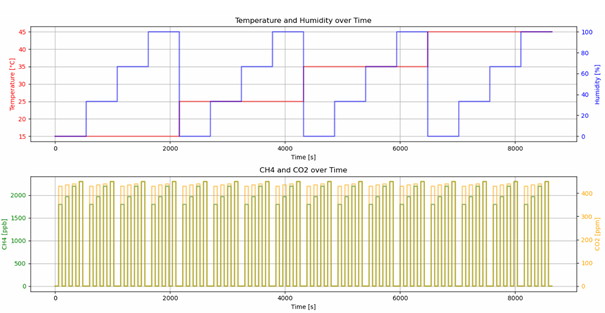
\includegraphics[width=\textwidth]{0_images/figures/calibrationProfile.png}
    \caption{Preliminary calibration profile to collect training data at Norunda.}
    \label{fig:calibration_profile}  
\end{figure}



%The focus of attention for \gls{mirage} is to demonstrate the %applicability of the \gls{ndir} sensor for low-cost and low-complexity %methane measurements in the stratosphere.
%Since the biggest trade-off is resolution in this endeavour, the %uncertainty of the measurement will be assessed with great care.
%A lot of this will be done before the flight by carefully calibrating the %sensor in the temperature and pressure range of the measurement chamber %for different methane concentrations and humidity levels.
%If possible, a machine learning algorithm will be trained to reduce the %impact of noise on the measurements, similar to \cite{gia_accurate_2025}. %This is an important prerequisite for the quality of the data collected %during the flight.

%To further demonstrate the reliability of the measurement data, the focus %of post-flight data analysis is on comparison of the vertical methane %profile from ascent and descent with other sources of methane data.
%For this it is intended to use:

%\begin{enumerate}
%    \item Radiative transfer models (like RTTOV)
%    \item Chemistry and Transport models (like MOCAGE)
%    \item Satellite data
%    \item In-situ measurement data from other groups
%\end{enumerate}

%\gls{rtm} like RTTOV can provide reference concentration profiles of %atmospheric gases like methane and have been compared to \gls{tdlas} %measurements before.
%\gls{ctm} like MOCAGE assimilate satellite data into their calculations %and give an additional gauge of what should be expected for the data %collected by MIRAGE, although they have shown worse correspondence with %in-situ measurements \cite{joly2020}.
%The use of satellite data in addition to their indirect use via \gls{ctm} %needs to be assessed.
%This and the familiarisation with \gls{rtm} and \gls{ctm} will be part of %a bachelor thesis project within \gls{mirage}, that is planned for several %team members.
%
%In-situ measurements were conducted with \gls{tdlas} from ESRANGE in 2016 %and provide a direct comparison with more expensive but also more accurate %laser-based methods \cite{Khair2017}.
%The comparison is of course limited because of the different times at %which measurements were done.
%It is still expected to get some interesting insights by including these %sources into the data analysis.
%Another in-situ measurement campaign conducted over France with AirCore in %2018 compared their data to \gls{ftir} measurements \cite{RINGO}.
%This is an interesting study for us as well, especially if ESRANGE can support us with LIDAR methane measurements.
%Whether this is possible is not clear yet but will be asked for.

%As a secondary goal we want to investigate, whether a correlation between %different landscapes and methane levels in the stratosphere can be drawn.
%Depending on the quality of our data and number of data points we collected %during the floating phase of the flight, we will study fluctuations and %compare them with the GPS data collected by the balloon.
%Since freshwater bodies, wetlands and industrial areas have higher methane %emissions than for example forests, we are interested whether methane %fluctuations in the stratosphere can be related to those different landscapes.
%Machine learning might be employed to help recognising those fluctuations.



%%%%%%%%%%%%%%%%%%%%%%%%%%%%%%%%%%%%%%%%%%%%%%%%%%%%%%%%%%%%%%%%%%%%%%%%%%%%%%%
\section{Launch Campaign}

This will be filled out in later versions of the \gls{sed}.

%%%%%%%%%%%%%%%%%%%%%%%%%%%%%%%%%%%%%%%%%%%%%%%%%%%%%%%%%%%%%%%%%%%%%%%%%%%%%%%
\section{Results}

Because of the pressure requirements that follow from the high limit of detection (LoD) of the K96 of about 3\,ppm it is expected that the data points will have less vertical resolution than in other in-situ missions. The measurement uncertainty of the concentration values will be also larger but if the calibration was done with the intended thoroughness, the results should be at least comparable to the different validation sources specified above. The working principle of the calibration has been proven in \cite{gia_accurate_2025} and shown very good results for the laboratory data. It should be noted however that the performance was significantly less for field studies and that the setup used by Gia et al. allowed for more precise calibration. The outcome is therefore uncertain but together with the whole data analysis pipeline, which takes the context of the data acquisition into account via quality flagging, it should be possible in the end to make at least a definitive assessment of the success of MIRAGE. \\
The resulting expectations for every objective for MIRAGE are summarised below in \tref{tab:mission_success}.

\begin{table}[H]
\centering
\caption{Mission Success}
\label{tab:mission_success}
\begin{tabularx}{0.9\textwidth}{p{2cm}p{5cm}p{5cm}}
\toprule
\textbf{Priority} & \textbf{Description} & \textbf{Expectation before CDR} \\
\midrule
Technical - Primary & Measure methane, carbon dioxide and water with an NDIR sensor core up to at least 20\,km altitude. & Should be reached but for $CH_4$ only with an uncertainty larger than 0.5\,ppm. \\
Technical - Primary & Demonstrate a pressurisation system that can maintain 3 bar up to at least 20\,km altitude.& Should be reached \\
Scientific - Secondary & Validate recorded measurements via chemical transport models, satellite data and previous in-situ measurements by other groups.& Depends on the first objective \\
Scientific - Secondary & Evaluate decrease of measurement uncertainty in the field by employing AI-based calibration. & Should be reached but unknown how much decrease of uncertainty \\
\bottomrule
\end{tabularx}
\end{table}



%There is a small chance that fluctuations of methane in the stratosphere can %be connected to the emissions at ground level even if very precise %measurement techniques are given. Especially, if we fly over different large %areas like wetlands or lakes and forests, we might be able to detect changes %in concentrations. Even if this goal fails, we will have collected methane %concentration data with higher accuracy at about 25-30 km height due to the %longer measurement time.

%%%%%%%%%%%%%%%%%%%%%%%%%%%%%%%%%%%%%%%%%%%%%%%%%%%%%%%%%%%%%%%%%%%%%%%%%%%%%%%
\section{Input to Campaign Report}

This section will be filled after the Campaign.

%%%%%%%%%%%%%%%%%%%%%%%%%%%%%%%%%%%%%%%%%%%%%%%%%%%%%%%%%%%%%%%%%%%%%%%%%%%%%%%
\section{Lessons Learned}

As a fresh and still growing team there were some lessons learned already. 
\begin{enumerate}
  \item It took too much time to recruit new team members and key team members are still missing; for example in software design.
  \item Wrong assumptions regarding the accuracy of the K96 sensor were made early one. This should have been prevented by asking more questions earlier on and closer communication with our contacts from Senseair AB.
  \item Holidays and more generous time estimates need to be taken into consideration to prevent finishing crucial project steps like the \gls{sed} under pressure, which can lead to worse quality.
  \item It it important to keep track of progress and check in with each sub team or team members working on specific tasks to prevent delays.
\end{enumerate}
Of course there are many more lessons of more practical nature. Everyone knows a little more about pumps and their limitations now, everyone learned something about methane sensing and many more things like that. However, the biggest lesson is probably that the documentation for such a project takes a lot of time and thought but also makes you aware of many aspects that can be easily overlooked.

%%%%%%%%%%%%%%%%%%%%%%%%%%%%%%%%%%%%%%%%%%%%%%%%%%%%%%%%%%%%%%%%%%%%%%%%%%%%%%%